\documentclass[9pt]{beamer}
\usetheme{CambridgeUS}


%\setbeamertemplate{headline}{}
\setbeamertemplate{navigation symbols}{}
\setbeamertemplate{section in head/foot shaded}[default][100]
\setbeamertemplate{mini frame in other subsection}{%
    \begin{pgfpicture}{0pt}{0pt}{0.1cm}{0.1cm}%
        \pgfpathcircle{\pgfpoint{0.05cm}{0.05cm}}{0.05cm}%
        \pgfusepath{fill,stroke}%
    \end{pgfpicture}%
}

\newcommand\blfootnote[1]{%
  \begingroup
  \renewcommand\thefootnote{}\footnote{#1}%
  \addtocounter{footnote}{-1}%
  \endgroup
}


\usepackage{comment} %% 20230510添加,\begin{comment} #1 \end{comment} 中内容不会编译显示。beamer无法直接加载此包,需要在\begin{frame}后添加属性[fragile]

\usepackage{textcomp}



\usepackage{booktabs}
\usepackage{ccicons}
\usepackage{mathrsfs}
\usepackage{ulem}
%%%%% 280622 ajoute
\usepackage{import} % 引入子文件
\usepackage{ragged2e} % 英文两端对齐
%%%%% 280728 ajoute
\usepackage[outline]{contour} % 字体加粗
\usepackage{multicol} % 分栏
\usepackage{xspace}
\newcommand{\themename}{\textbf{\textsc{metropolis}}\xspace}
\usepackage{physics}
\usepackage{tikz}
\usetikzlibrary{positioning, shapes.geometric}
\usetikzlibrary{graphs, positioning, quotes, shapes.geometric}


\definecolor{ChimieBlue}{RGB}{60,23,61}
\definecolor{molle}{RGB}{254,241,199}
\definecolor{amber}{rgb}{0.31, 0.78, 0.47}
%\setbeamertemplate{footline}[frame number] %% 添加页码


%\usepackage{mathptmx}
%\usepackage{anyfontsize}
%\usepackage{t1enc}
%自定义字体大小,以上来自https://texblog.org/2012/08/29/changing-the-font-size-in-latex/


\usepackage{textpos}
\addtobeamertemplate{footline}{}{
%\begin{textblock*}{100mm}(0.0\textwidth,-1.3cm) 
%%%\includegraphics[height=1.2cm]{LOGO/logo_all.png}
%\includegraphics[height=1.2cm]{LOGO/titre_haut.png}
%\end{textblock*}
\begin{textblock*}{100mm}(0.92\textwidth,-1.3cm) 
\countnumber
\end{textblock*}
} %%%%% 0.02横向比例;-1cm纵向高度




%%%%%%%%%%%%%%%%%%%%%%%%%%%%%%%%%%%%%%%%

\newcommand{\tenspace}{\ \ \ \ \ \ \ \ \ \ }
\newcommand{\tens}{\ \ \ \ \ \ \ \ \ \ }
\newcommand{\fivespace}{\ \ \ \ \ }
\newcommand{\fives}{\ \ \ \ \ }


\newcommand{\sct}{\section}
\newcommand{\ssc}{\subsection}
\newcommand{\sss}{\subsubsection}
\newcommand{\parag}{\paragraph}
\newcommand{\beq}{\begin{equation}}
\newcommand{\eeq}{\end{equation}}
\newcommand{\bgn}{\begin{align}}
\newcommand{\ggn}{\end{align}}
%\newcommand{\egnn}{\end{align}}
\newcommand{\tlag}[1]{\tag{#1} \label{#1}}


\newcommand{\mrm}{\mathrm}
\newcommand{\bb}[1]{\mathbb{#1}} %% 空心大写字母
\newcommand{\bbf}[1]{\mathbf{#1}} %% 黑体向量
\newcommand{\cal}{\mathcal} 
\newcommand{\scr}{\mathscr} %% 花体字母
\newcommand{\wtd}{\widetilde}


\newcommand{\pder}[2][]{\frac{\partial#1}{\partial#2}}


\newcommand{\llp}{\left(}
\newcommand{\rrp}{\right)}
\newcommand{\lls}{\left[}
\newcommand{\rrs}{\right]}
\newcommand{\llc}{\left\{}
\newcommand{\rrc}{\right\}}
\newcommand{\lld}{\left.}
\newcommand{\rrd}{\right.}
\newcommand{\lla}{\left\langle}
\newcommand{\rra}{\right\rangle}
\newcommand{\llang}{\left\langle}
\newcommand{\rrang}{\right\rangle}
\newcommand{\llv}{\left\vert}
\newcommand{\rrv}{\right\vert}
\newcommand{\uu}{\underline}
\newcommand{\tit}{\textit}
\newcommand{\tbf}{\textbf}
\newcommand{\eq}[1]{\begin{equation} #1 \end{equation}}
\newcommand{\agn}[1]{\begin{align} #1 \end{align}}


\newcommand{\eps}{\epsilon}
\newcommand{\veps}{\varepsilon}
\newcommand{\varphi}{\vph}
\newcommand{\al}{\alpha}
\newcommand{\bt}{\beta}
\newcommand{\ab}{\alpha\beta}
\newcommand{\dlt}{\delta}
\newcommand{\Dlt}{\Delta}
\newcommand{\gma}{\gamma}
\newcommand{\kpa}{\kappa}
\newcommand{\kxi}{\kappa\xi}
\newcommand{\kxe}{\kappa\xi\epsilon}
\newcommand{\tta}{\theta}

















\title[Audition ED IP Paris - Concours commun]{
\Huge Audition ED IP Paris - Concours commun \\
\bigskip
\hline \\
\bigskip
\Large \tbf{Probabilistic Approach to Diffusion-Mediated Surface Phenomena}}
\author[Y. YE]{\large Director: \tbf{Denis GREBENKOV} \\
\normalsize
Laboratoire PMC, Ecole Polytechnique}

\date[May 15, 2023]{\large{\tbf{Yilin YE}} \\
\normalsize May 15, 2023}

\begin{document}

\begin{frame}[noframenumbering,plain] 
%% noframenumbering = \addtocounter{framenumber}{-1}
%% plain = \thispagestyle{empty}
\titlepage
%\addtocounter{framenumber}{-1} %% 首页页码设定为-1,则下一页页吗变为+1
%\thispagestyle{empty} %% 首页不显示页脚
\end{frame}






\section{Curriculum Vitae}
\begin{frame}[fragile]
	\frametitle{\tbf{Academic Training}}
	
	\begin{comment}
	%%%
	\begin{minipage}{0.1\linewidth}
	
	\begin{center} \begin{tabular}{c}
	
\includegraphics[height=1 cm]{logos/logoxmu.png} \\
	
\includegraphics[height=1 cm]{logos/logoens.png} \\
	
\includegraphics[height=1 cm]{logos/Hunan_University_logo.png} \\
	
\includegraphics[height=1.1 cm]{logos/chimie.png} \\
%	
\includegraphics[trim={25cm 5cm 0 5cm},clip,height=0.8cm]{logos/ENS_Dpt_Chemistry_Logo.png} \\
	
\includegraphics[height=1 cm]{logos/hiboux.jpeg}
	\end{tabular} \end{center}
	
	\end{minipage}
	\end{comment}


	\begin{itemize}
	\setlength{\itemsep}{12pt}
	\item[$\bullet$] Undergraduate, Chemistry. \hfill 2015 - 2019 \\
		\textit{Xiamen University, Xiamen, China} \hfill \textbf{92.34}/100
		
	\item[$\bullet$] Diplôme de l'ENS. (International Selection) \hfill 2019 - 2023  \\
		\textit{École Normale Supérieure, Paris, France} \hfill In progress

	\end{itemize}
	
	\bigskip

	%%%
	\begin{minipage}{0.06\linewidth}
	\textcolor{white}{Just for space}
	\end{minipage}
	%%%
	\begin{minipage}{0.93\linewidth}
	\begin{itemize}
		\setlength{\itemsep}{12pt}
			
	\item[$\star$] Research Assitant. \hfill 2020 - 2021  \\
		\textit{Hunan University, Changsha, China}
		
	\item[$\star$] Master 1, Chemistry. \hfill 2021 - 2022 \\
		\textit{École Normale Supérieure, Paris, France} \hfill \textbf{15.60}/20
		
	\item[$\star$] Master 2, Physics, ICFP. \hfill 2022 - 2023 \\
		\textit{École Normale Supérieure, Paris, France}
		\hfill (1st semester) \textbf{13.69}/20 \\
	\hfill (2nd semester, without internship) \textbf{15.00}/20
	\end{itemize}
	
	\end{minipage}
	
\end{frame}






\import{}{courses_select.tex}
\import{}{stage_select.tex}







\section{Internships}
\import{}{eff_friction_EDIPP.tex}
%\import{}{traj-2d-kpa_EDIPP.tex}










\section{Thesis}
\frame{
	\frametitle{\tbf{Thesis Project - Motivation}}
	%%%
	\begin{minipage}{0.52\linewidth}
	\begin{center}
	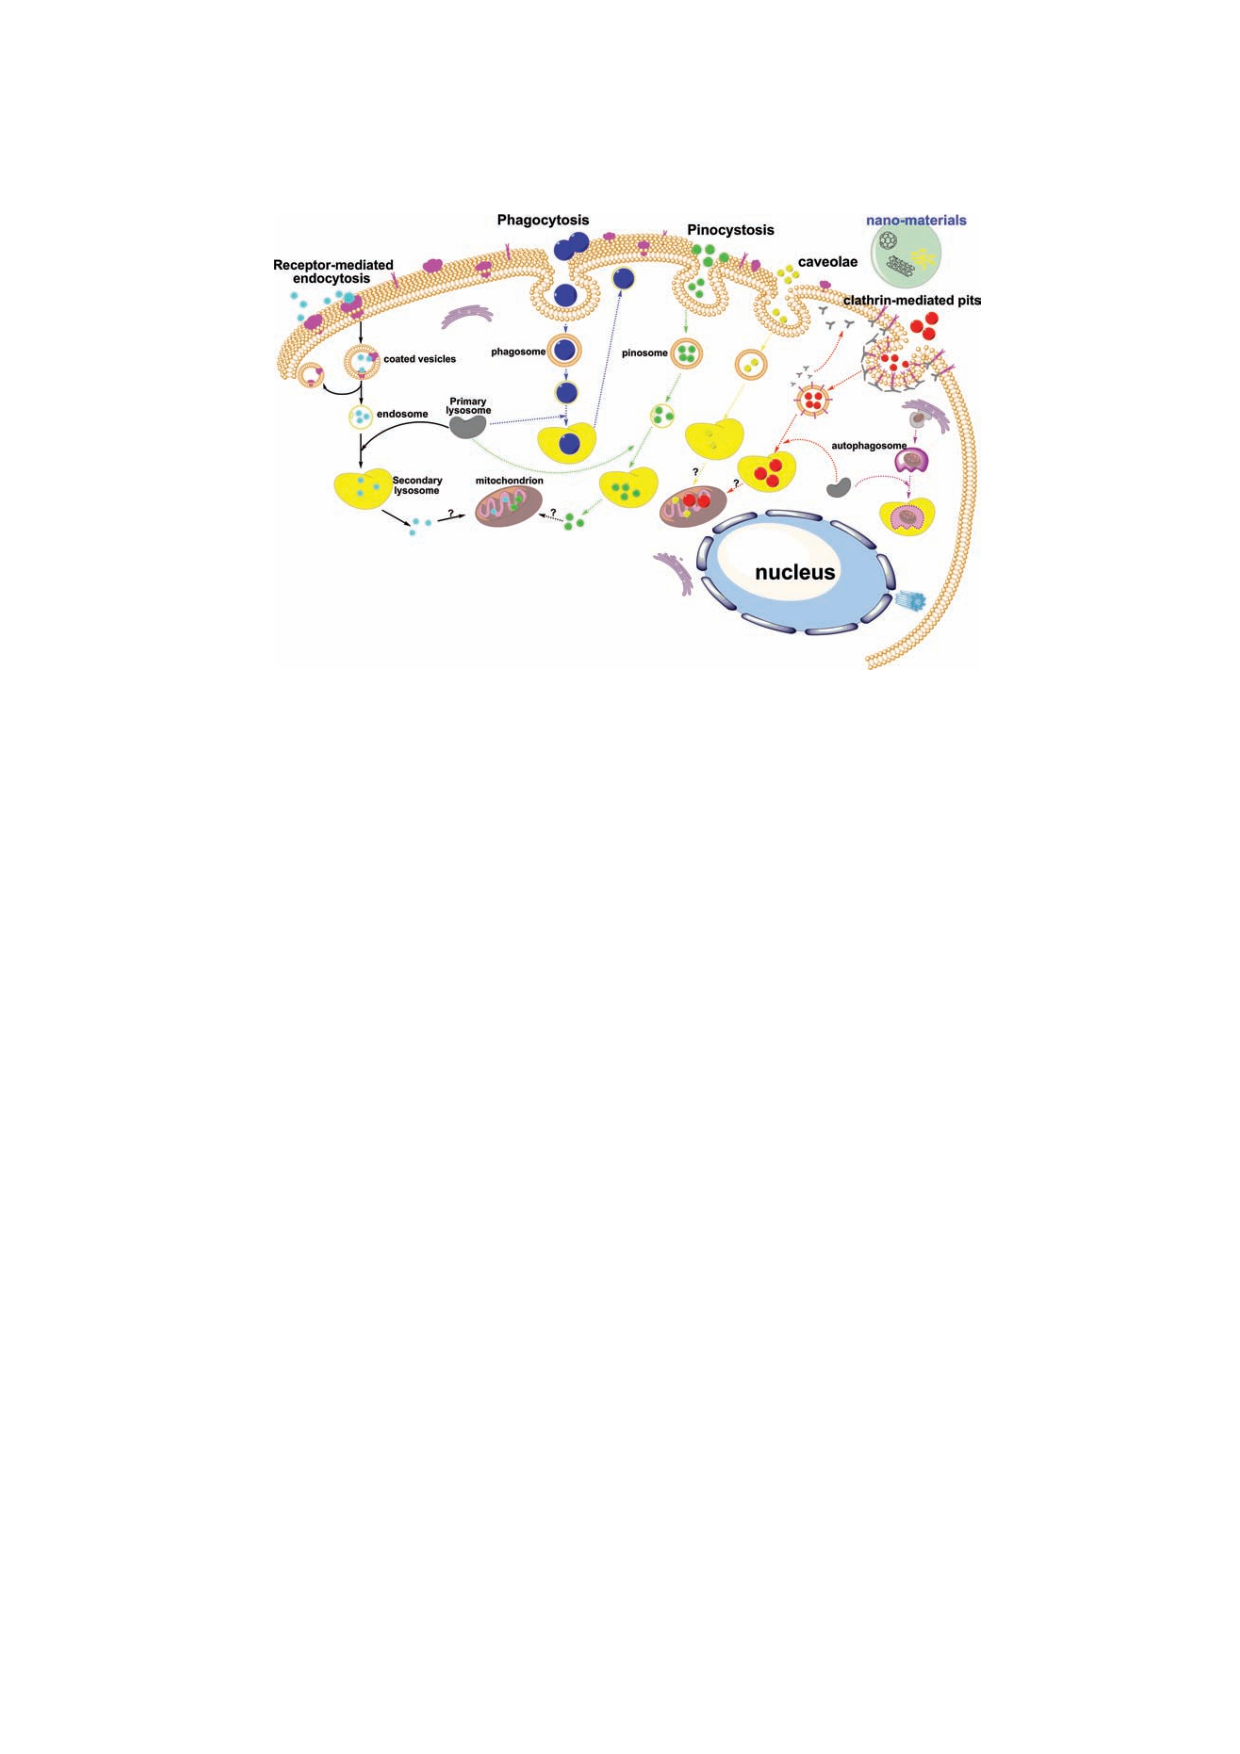
\includegraphics[height=4cm]{figs/zhao2011_fig1.pdf}
	\end{center}
	\end{minipage}
	%%% 注意加%避免换行
	\begin{minipage}{0.4\linewidth}
	\begin{center}
	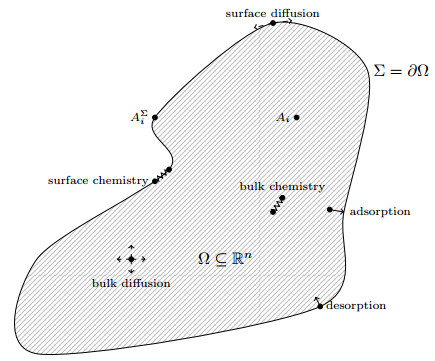
\includegraphics[height=4.5cm]{figs/surf_chem.jpg}
	\end{center}
	\end{minipage}

\bigskip

	\begin{center}
	\Large
	\tbf{How does the complicated environment \\ affect diffusion-controlled reactions?} 
	\end{center}
	
	\blfootnote{B. Augner, and D. Bothe. arXiv:1911.13030, \tbf{2019}}
	\blfootnote{F. Zhao, et al. \tit{Small}, \tbf{2011}, \tit{7}(10), 1322-1337}
}






\begin{frame}[fragile]
  \frametitle{\tbf{Thesis Project}\\
  \small{Probabilistic Approach to Diffusion-mediated Surface Phenomena}}


\large
\begin{comment}
  \begin{itemize}
    	\setlength{\itemsep}{6pt}
%    \item Construct general model with Encounter-based approach
    \item \tbf{Local Time} $\ell$ describes the general nature of surface phenomena: ``target-finding'' diffusion, activation, passivation, etc.   %How much time would one particle move near the complex surface?
    \item Implement ``encounter-based approach'' in the complex media with special geometrical confinements;% for $P(\mathbf{x},\ell,t|\mathbf{x}_0)$
  \item Study different mechanisms of surface reactions 
  %with generalized propagator $G_\Psi(\mathbf{x},t|\mathbf{x}_0) = \int \mrm{d} \ell \Psi(\ell) P(\mathbf{x},\ell,t|\mathbf{x}_0)$ 
  by ``encouter-dependent reactivity''; 
  %\item Collective effect of multiple independently diffusing particles;
  \item Identify experimental situations to validate;
  \end{itemize}
\end{comment}



	\begin{itemize}
	    	\setlength{\itemsep}{6pt}
		\item[$\bullet$] Boundary local time $\ell_t$ characterizes the number of encounters with the boundary
		\item[$\bullet$] Surface reaction occurs when $\ell_t$ exceeds some threshold $\hat\ell$ characterized by $\Psi(\ell)$
		\large
		\begin{itemize}
          \item[$\star$] standard surface reactions $\Psi(\ell) = q e^{-q\ell}$
          \item[$\star$]  various surface reactions: arbitrary $\Psi(\ell)$
        \end{itemize}
		\item[$\bullet$] This approach was applied only in simple confinements like sphere.
	\end{itemize}

\begin{center}
\includegraphics[height=3cm]{figs/pending_scheme.png}
\end{center}
  
  %\blfootnote{Y. Zhou, et al. Comm. Math. Sci., 15, 237-259 (2017).}
  %\blfootnote{Y. Lanoiselée, et al. Nature Commun. 9, 4398 (2018).}
  \blfootnote{D. S. Grebenkov, Physical Review Letters 125, 078102 (2020)}
  
  
\end{frame}





\frame{
	\frametitle{\tbf{Thesis Project - Aims} \\
	  \small{Probabilistic Approach to Diffusion-mediated Surface Phenomena}}

	
	\large
  \begin{itemize}
  	\setlength{\itemsep}{8pt}
%  \item Efficient numerical methods towards different cases;
  \item Numerical practices on local time and conditional probability $P(\mathbf{x},\ell,t|\mathbf{x}_0)$;
  %diffusion on the surface;
  \item Analyze reversible chemical reactions by generalized propagator $G_\Psi(\mathbf{x},t|\mathbf{x}_0) = \int \mrm{d} \ell \Psi(\ell) P(\mathbf{x},\ell,t|\mathbf{x}_0)$;
  \item Popularize 2D model towards 3D model for simulations of real cases;
  \end{itemize}
  
  \begin{center}
  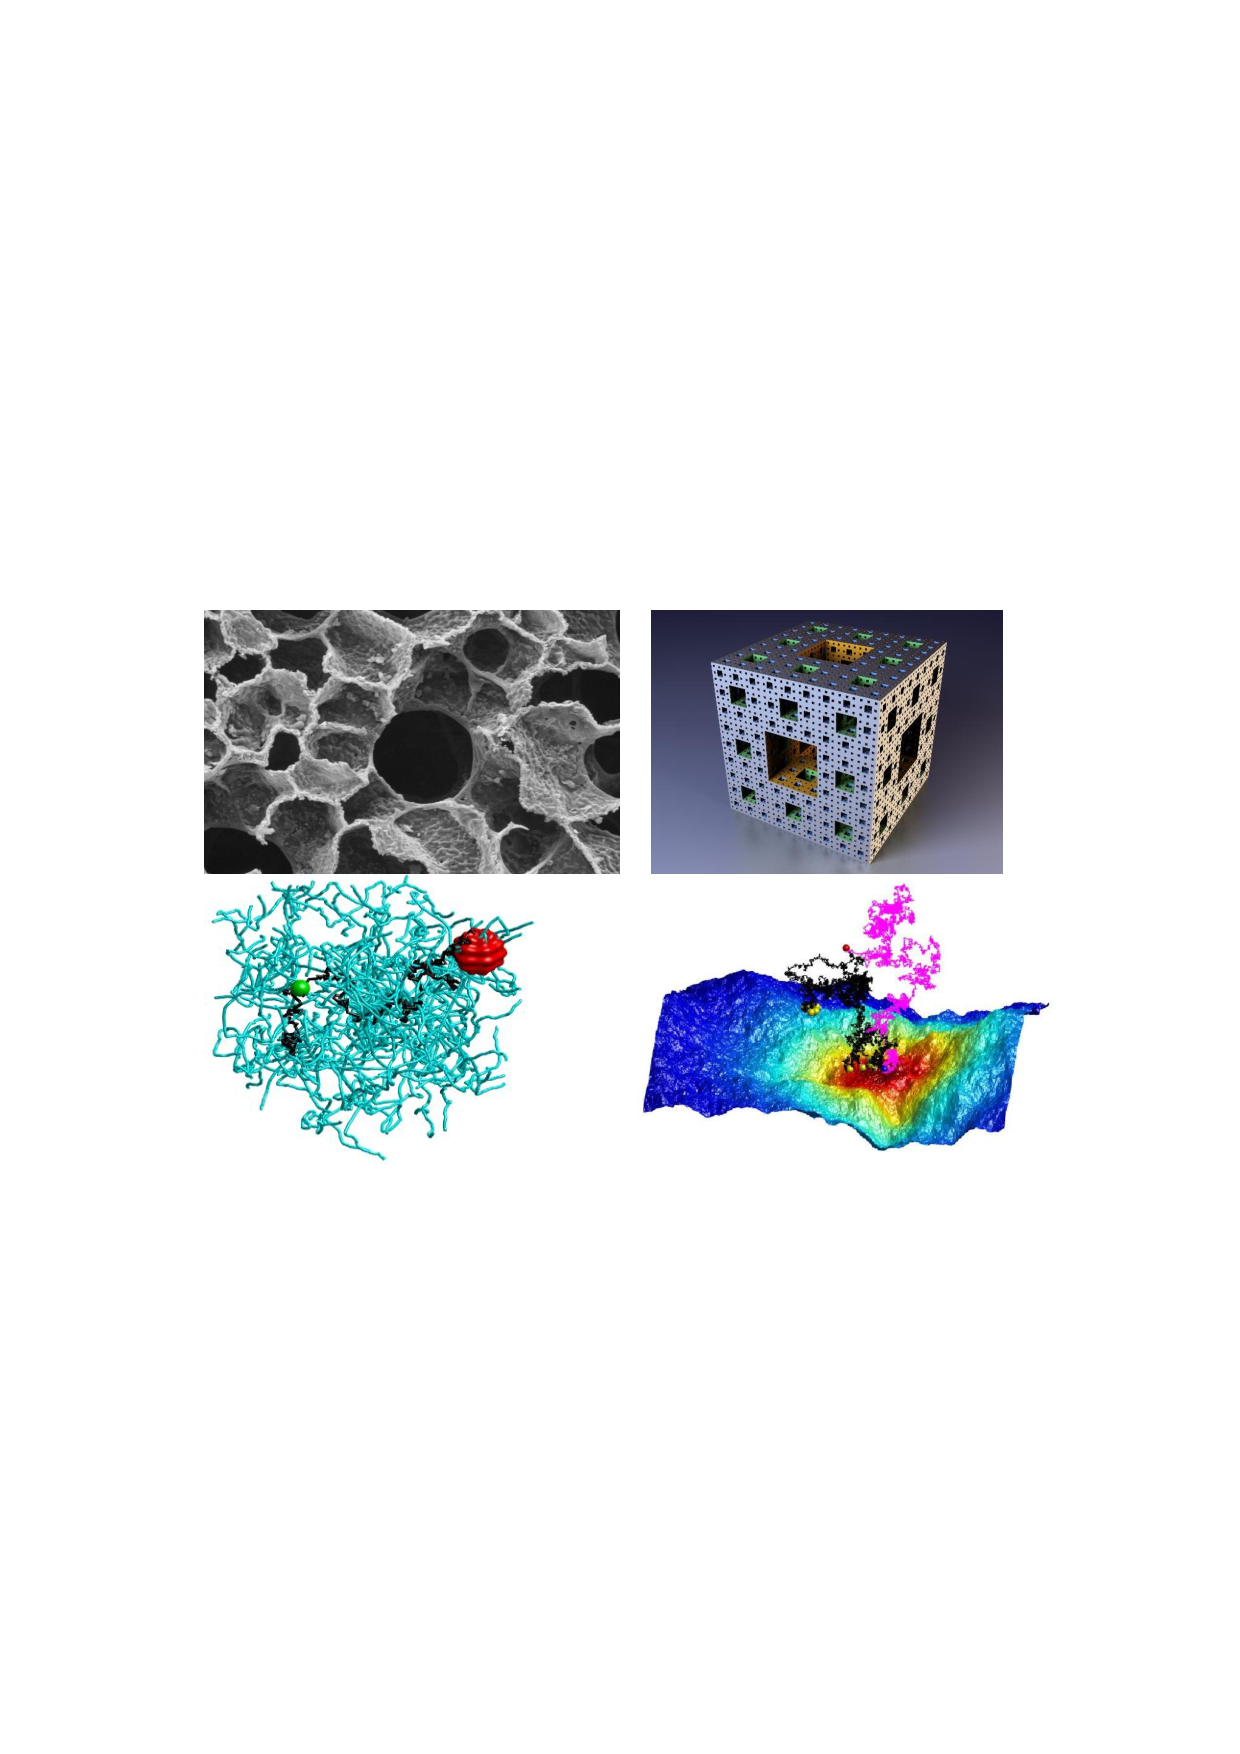
\includegraphics[height=3.6cm]{figs/PhD_project_final_figs.pdf}
  \end{center}
}






\begin{frame}
\frametitle{\tbf{Internship - M2} \\
\small{Brownian motion as Markov-chain Monte Carlo}}
%This page is left for alg details, comparing classical Brownian motion simulations and GAFRW.

		%%%
    \begin{minipage}{0.48\linewidth}
    	$$ \dlt = \mrm{constant} $$
        $$ \Dlt x_i = \mrm{ran}(-\dlt,+\dlt) \fives \Dlt y_i = \mrm{ran}(-\dlt,+\dlt) $$
    \begin{center}
    	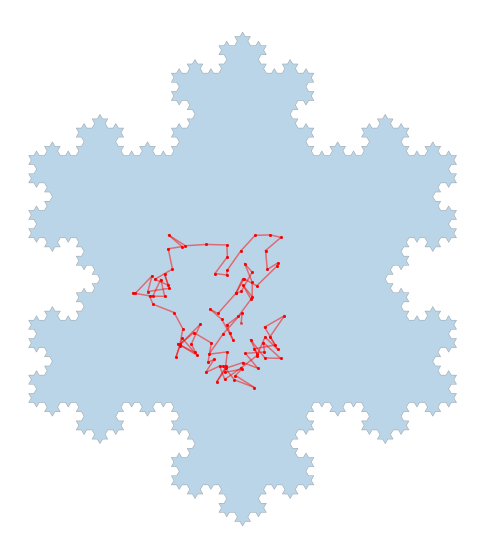
\includegraphics[height=6.4cm]{figs/diffuse_MCMC.png}
    \end{center}
    \end{minipage}
    	%%%
    \begin{minipage}{0.48\linewidth}
        $$ r = \mrm{constant} \fives \tta_i = \mrm{ran}(0,2\pi) $$
        $$ \Dlt x = r \cos\tta_i \fives \Dlt y = r \sin\tta_i $$
    \begin{center}
		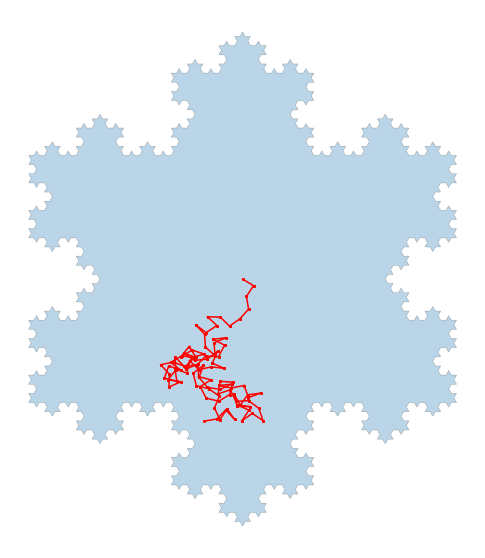
\includegraphics[height=6.4cm]{figs/diffuse_req.png}
    \end{center}
    \end{minipage}


\end{frame}






\frame{
	\frametitle{\tbf{Internship - M2} \\
	\small{Geometry-adapted fast random walk} }
		%%%
    \begin{minipage}{0.55\linewidth}
$$ r_i \neq \mrm{constant} \fives \tta_i = \mrm{ran}(0,2\pi) $$
%$$ \Dlt x_i = r \cos\tta_i \fives \Dlt y_i = r \sin\tta_i $$
    \begin{center}
        Find maximal radius and Jump uniformly. \\
    	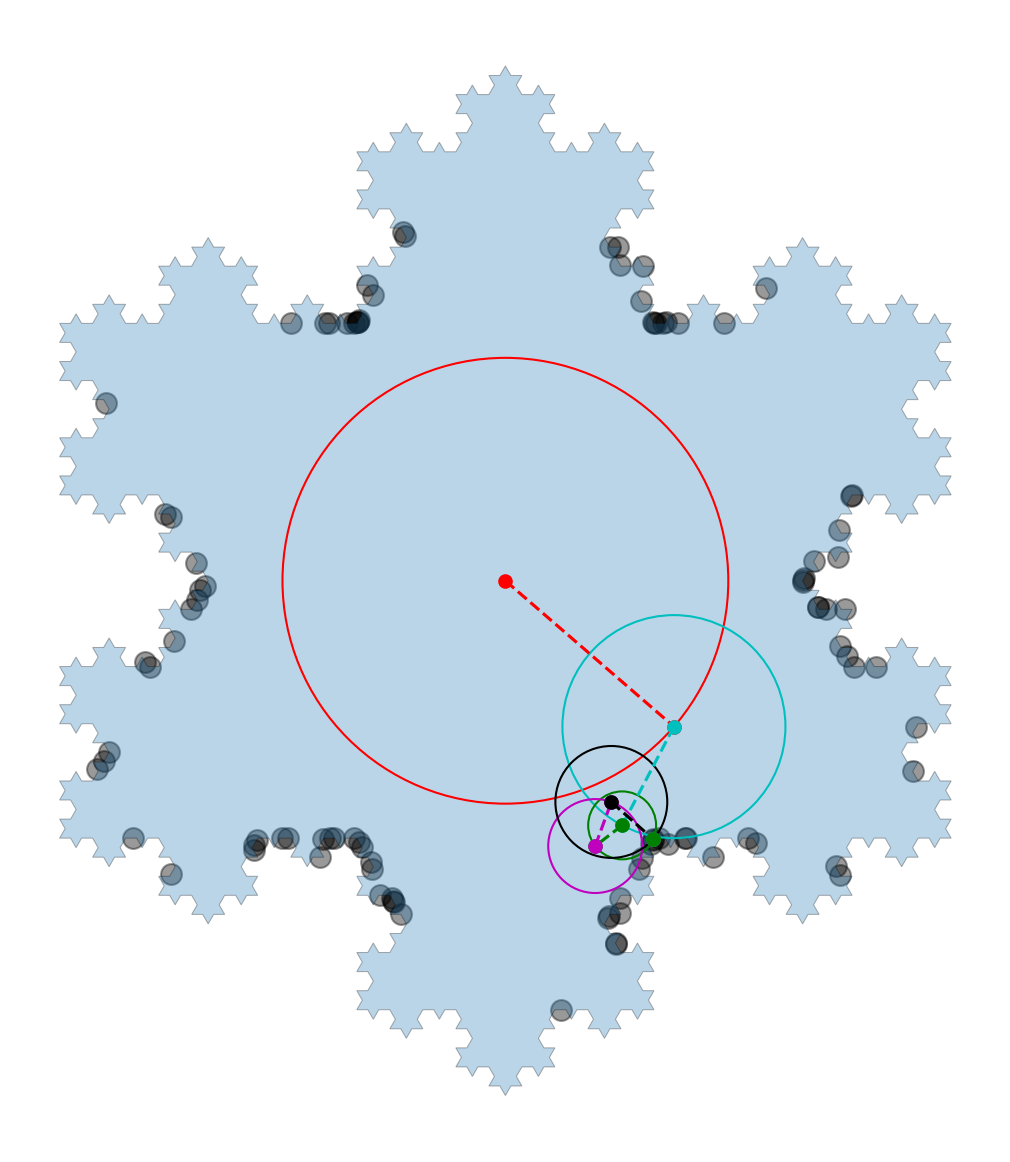
\includegraphics[height=6cm]{figs/GAFRW_g4.png}
    \end{center}
    \end{minipage}
    	%%%
    \begin{minipage}{0.4\linewidth}
    \begin{center}
    Compute distribution probability \\ on each segment:
    	%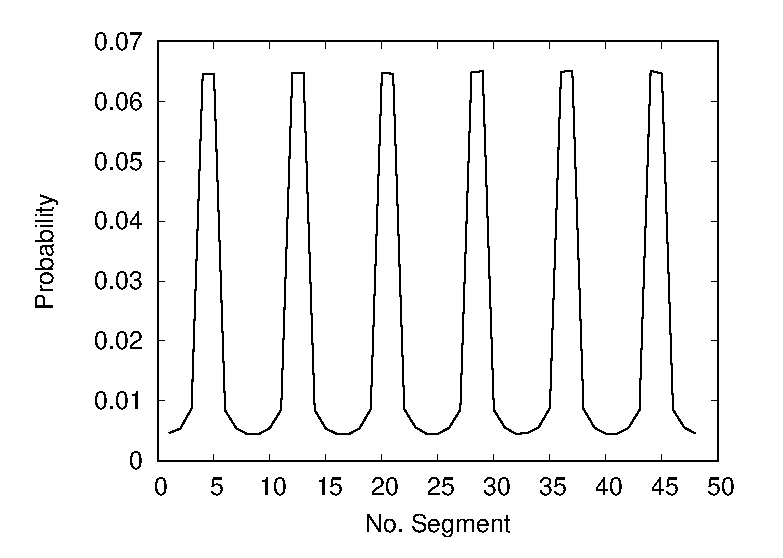
\includegraphics[height=3.6cm]{figs/pbbg2v3_EDIPP.eps}
	    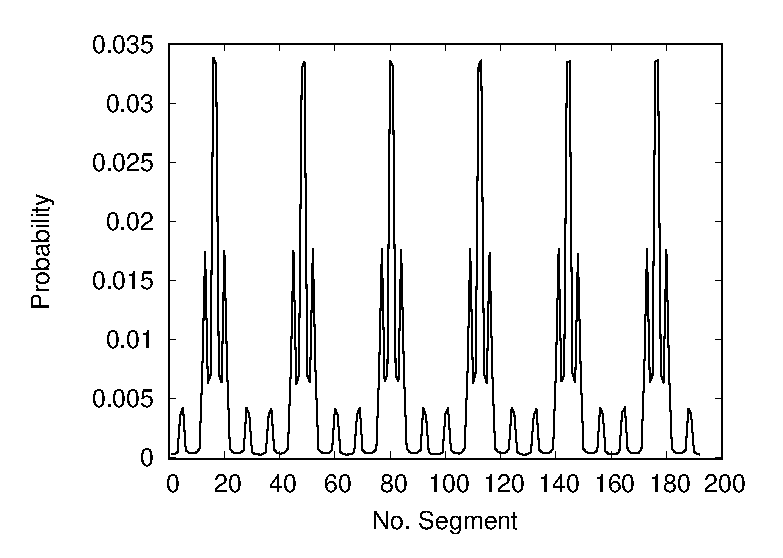
\includegraphics[height=3.2cm]{figs/pbbg3v3_EDIPP.eps}
    	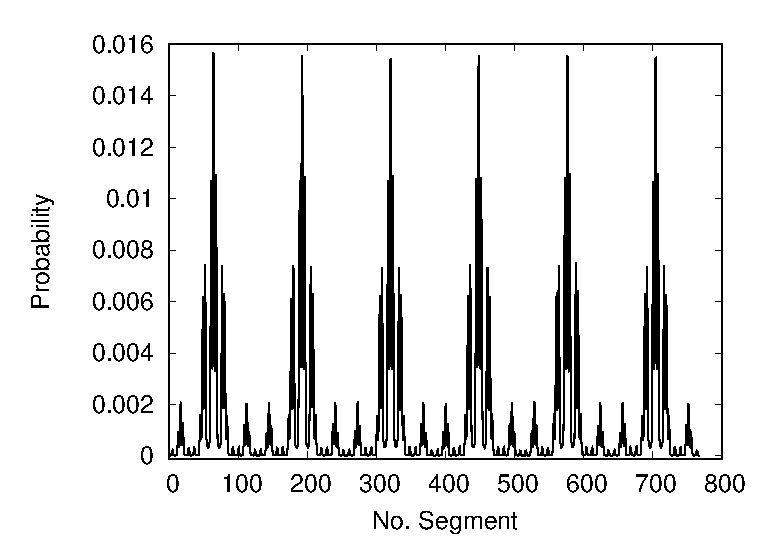
\includegraphics[height=3.2cm]{figs/pbbg4v3_EDIPP.eps}
    \end{center}
    \end{minipage}
    
\blfootnote{D. S. Grebenkov, et al. Physical Review E, 71(5), 056121 (2005).}
}






\section{}
\begin{frame}[noframenumbering]
\thispagestyle{empty}
	\begin{center}
	\textbf{\Huge{Thanks for your attention!}} \\[6ex]
	  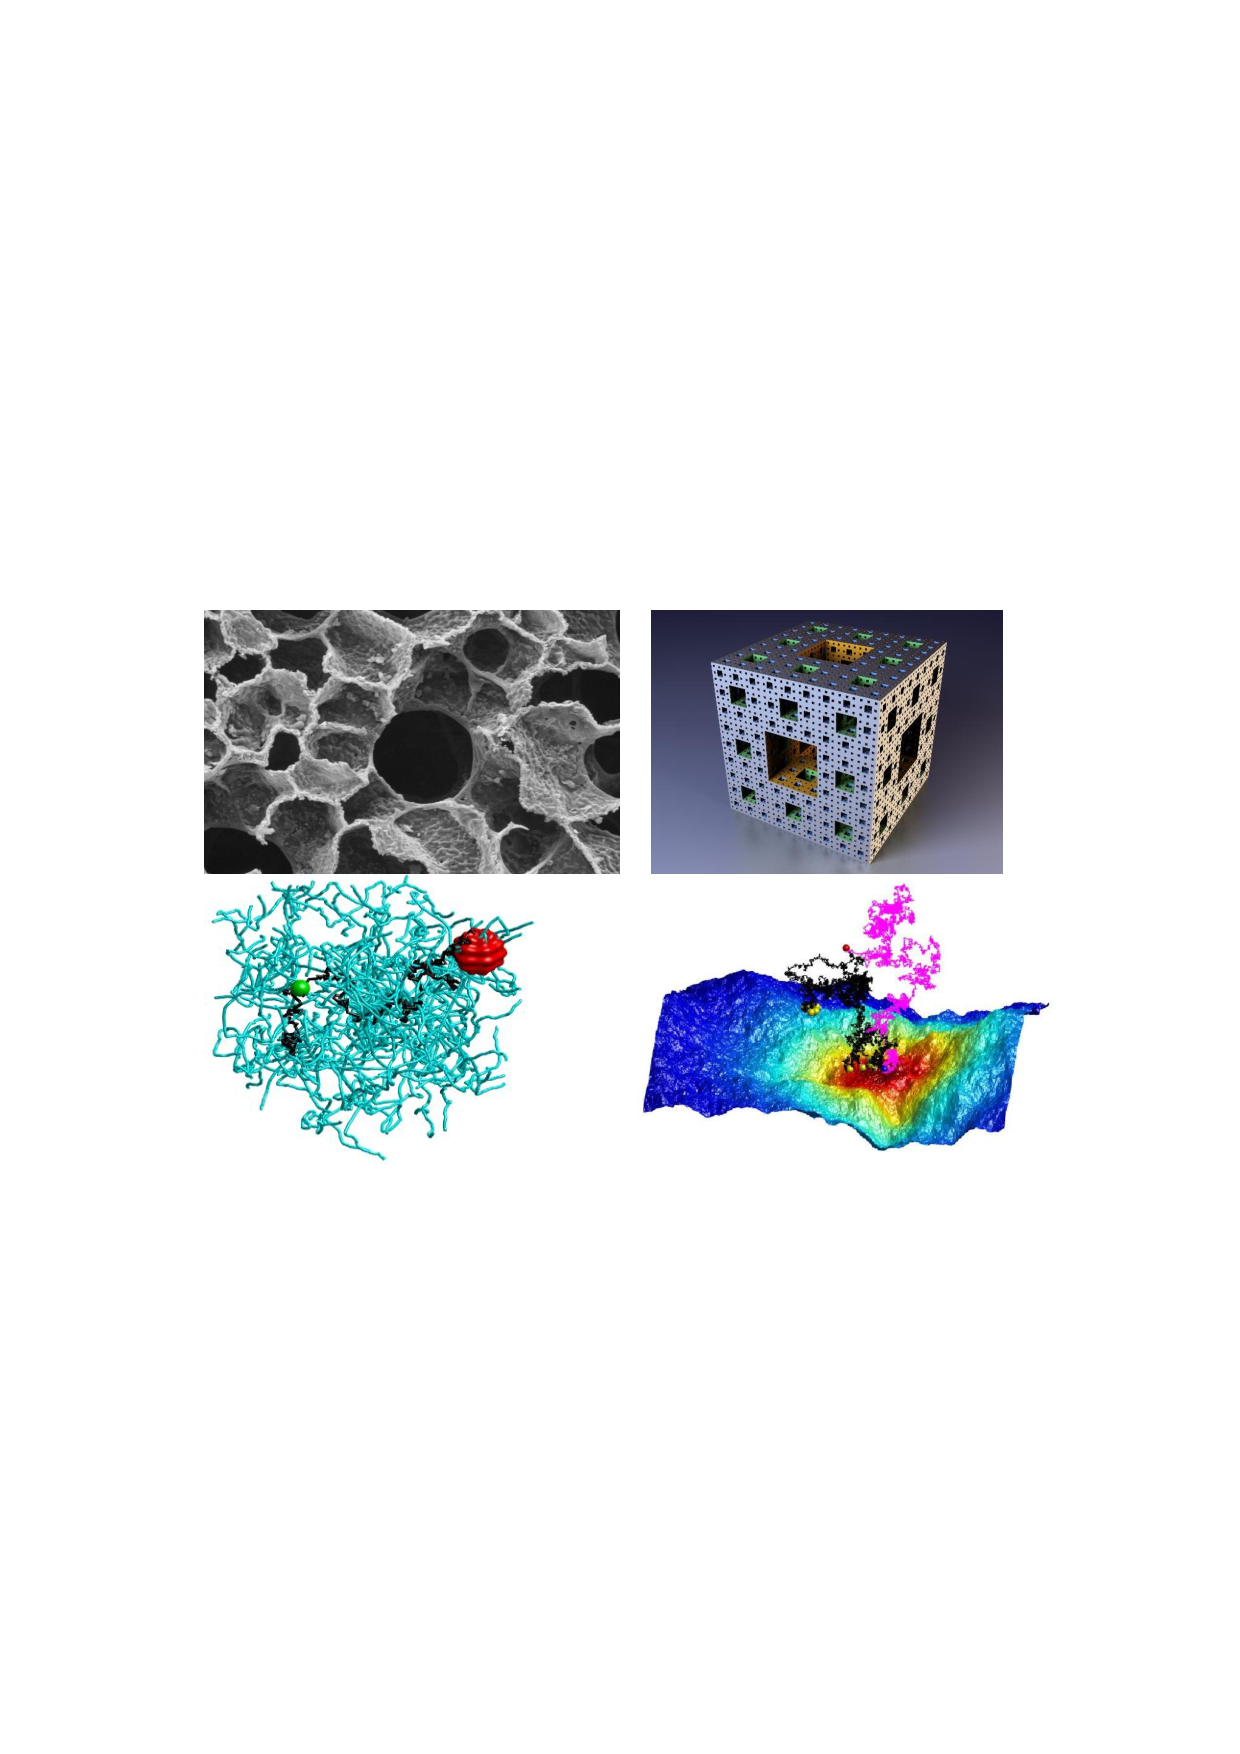
\includegraphics[height=4.5cm]{figs/PhD_project_final_figs.pdf}
	\end{center}
\end{frame}












\section{Appendix}
\begin{frame}[noframenumbering]
	\frametitle{}

	\begin{minipage}{0.65\linewidth}
		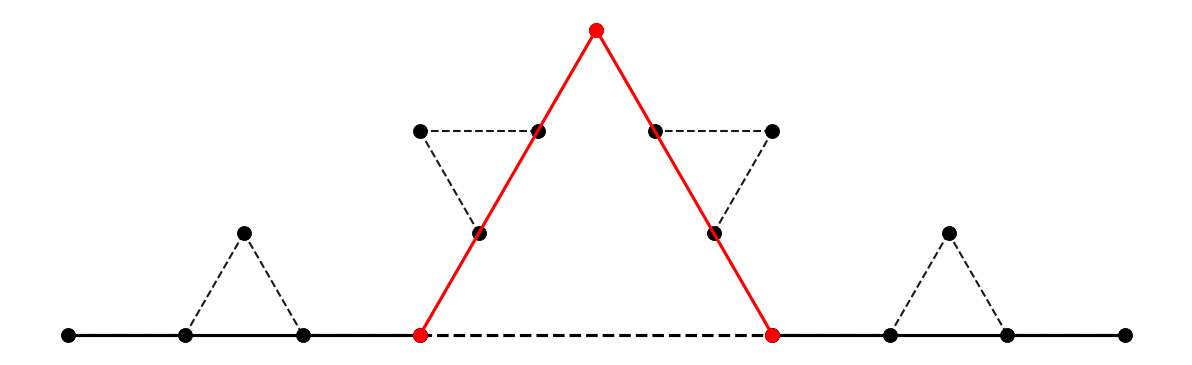
\includegraphics[height=2.5cm]{figs/no_ana.png}
	\end{minipage}
	%%%
	\begin{minipage}{0.33\linewidth}
		\Huge $$ P \llp \vdots \rrp \neq \sum P(\textcolor{red}{|}) $$
	\end{minipage}
	\begin{center}
    	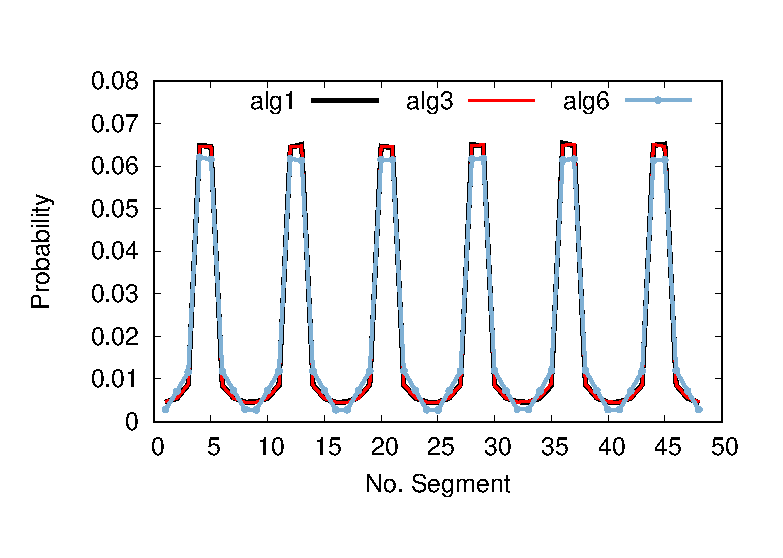
\includegraphics[height=6cm]{figs/pbb_g2_EDIPP.eps}
	\end{center}
\end{frame}





\begin{frame}[noframenumbering]
	\frametitle{}

	%%%
	\begin{minipage}{0.48\linewidth}
	\begin{center}
		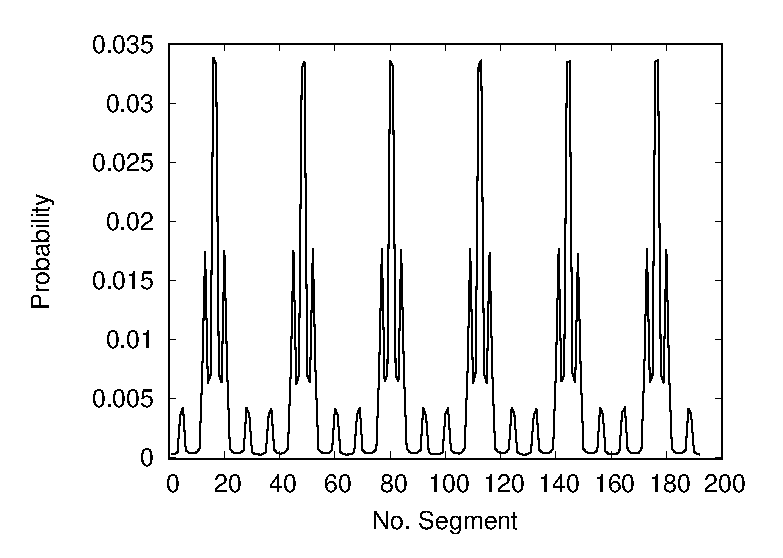
\includegraphics[height=4.2cm]{figs/pbbg3v3_EDIPP.eps}
		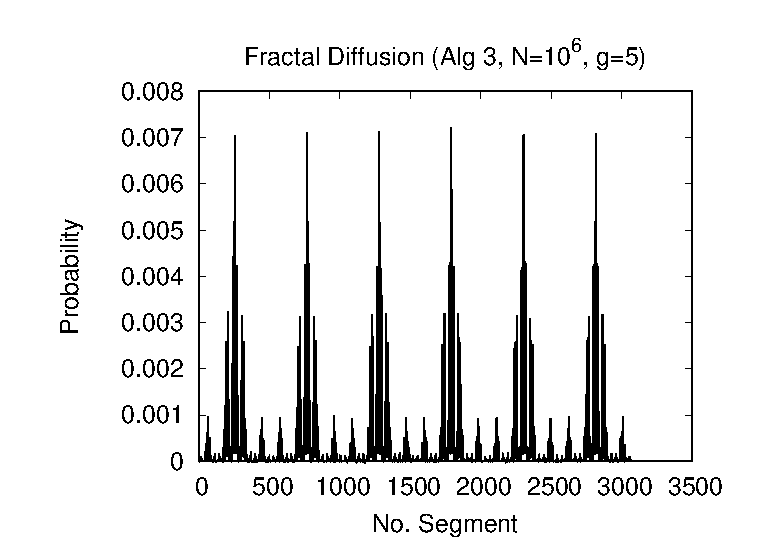
\includegraphics[height=4.5cm]{figs/pbbN1e6g5_v3.eps}
	\end{center}
	\end{minipage}
	%%%
	\begin{minipage}{0.48\linewidth}
	\begin{center}
		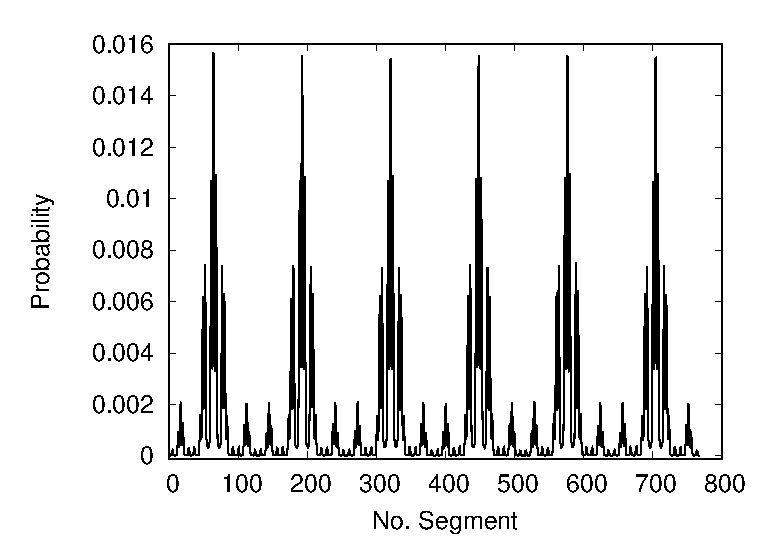
\includegraphics[height=4.2cm]{figs/pbbg4v3_EDIPP.eps}
    	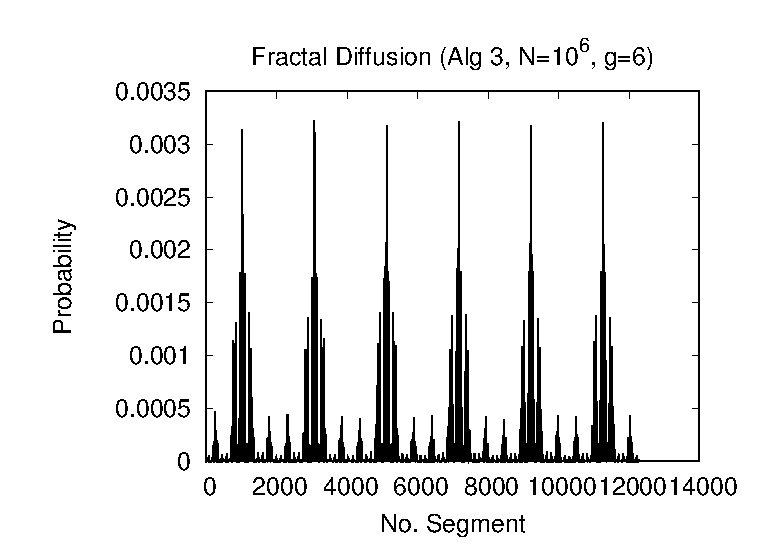
\includegraphics[height=4.5cm]{figs/pbbN1e6g6_v3.eps}
	\end{center}
	\end{minipage}
\end{frame}






\begin{frame}[noframenumbering]
	\frametitle{\tbf{Local Time} $\ell$}
	
  %%%
  \begin{minipage}{0.5\linewidth}
  $$ \vec{x}_{k+1} = \vec{x}_k + \rho(\cos\tta_, \sin\tta_k) $$
  
  $$ \tau = \frac{\dlt^2}{4D} \tens t_{k+1} = t_k + \tau $$
  
  $$ \ell_{t_{k+1}} = \ell_{t_k} + \sqrt{\frac{\pi}{2} D \tau} $$
  
  \end{minipage}
   %%%
  \begin{minipage}{0.4\linewidth}
  	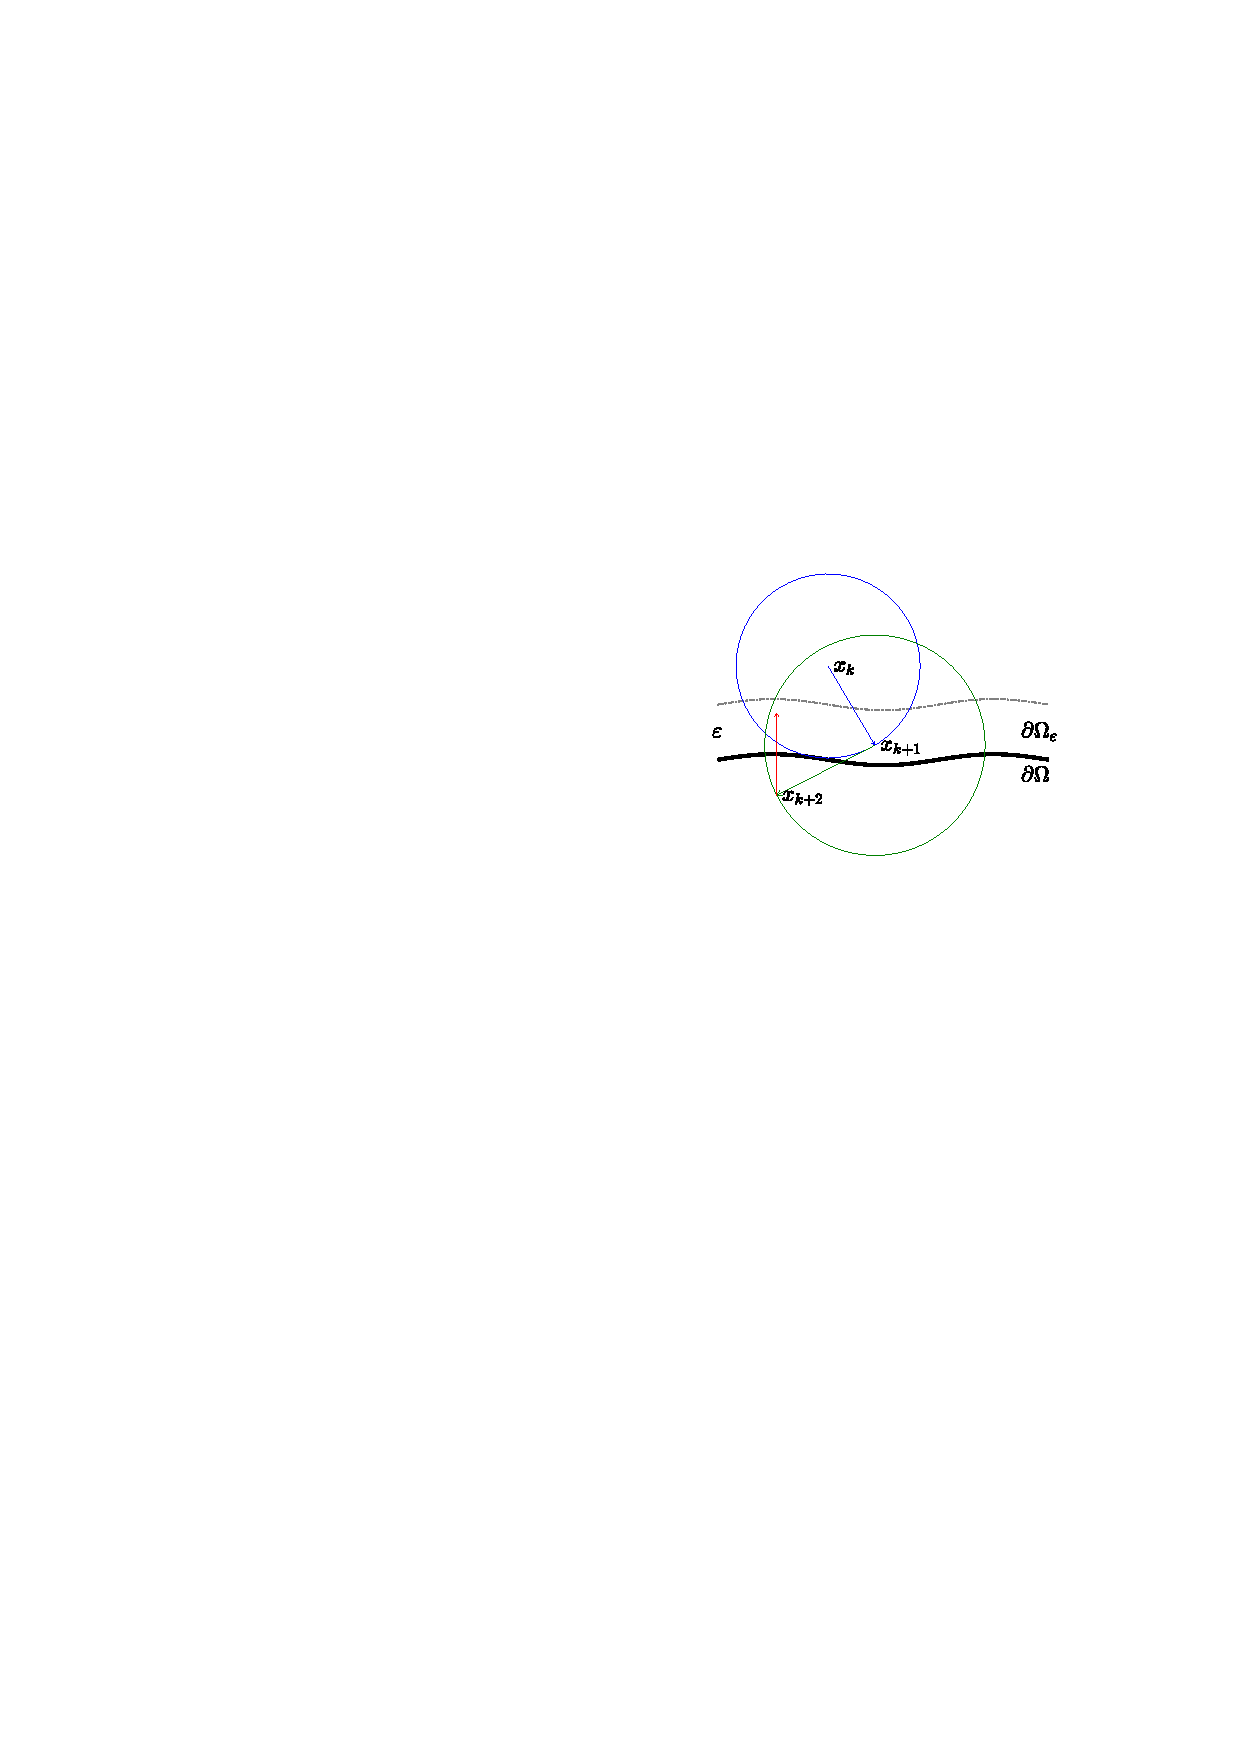
\includegraphics[height=4.5cm]{figs/simu_reflect.pdf}
  \end{minipage}
	
\end{frame}





\begin{frame}[noframenumbering]
	\frametitle{}

	\begin{center}
	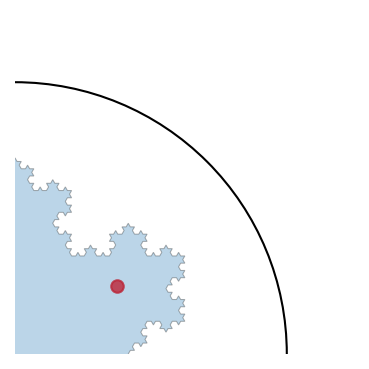
\includegraphics[height=4.0cm]{figs/int_convex.png}
	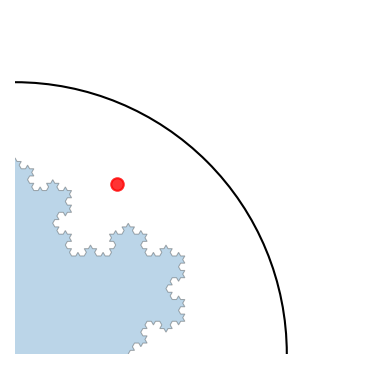
\includegraphics[height=4.0cm]{figs/ext_convex.png}
	\end{center}
	\begin{center}
	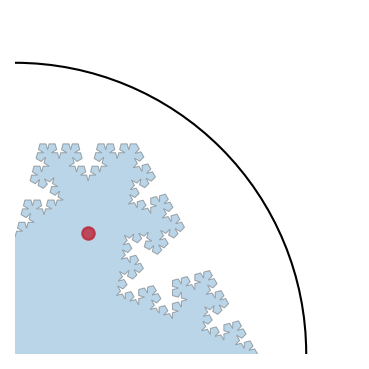
\includegraphics[height=4.0cm]{figs/int_concave.png}
	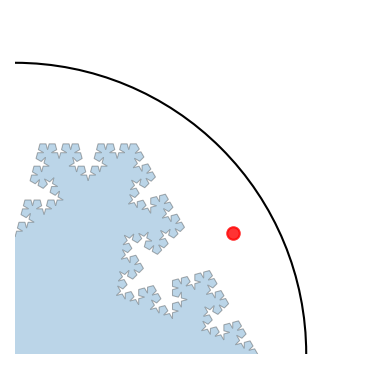
\includegraphics[height=4.0cm]{figs/ext_concave.png}
	\end{center}
	
\end{frame}





\begin{frame}[noframenumbering]




\end{frame}








\end{document}
